\documentclass[final,12pt,aspectratio=43]{beamer}
\usepackage[T1]{fontenc}
\usepackage{lmodern}
\usepackage[utf8]{inputenc}
\usepackage[english,ukrainian]{babel}
\usepackage{cite}
\usepackage{floatflt}
\usepackage{enumerate}
\usepackage{hyperref}
\usepackage{tabularx}
\usepackage{tikz}
\usepackage[pdftex]{graphicx}
\usepackage{color}
% \usetheme{Frankfurt}
% \usetheme{PaloAlto}
\usetheme{Dresden}
\usecolortheme{default}
\usefonttheme[onlymath]{serif}

\beamertemplatenavigationsymbolsempty
% \title{ Ідеї - то єдине, що в нас насправді є }
\title{Promis - проектування та огляд інструментарію}
% \author{Anatolii V. Koval${}^{1}$}
% \institute{${}^1$ Taras Shevchenko National University of Kyiv, Kyiv, Ukraine}

% \date{2011}

\begin{document}

% -------------------------------------------------- Defines ------------------
\definecolor{light-blue}{rgb}{0.8, 0.85, 1}

% --------------------------------------------------- Slide -------------------
\begin{frame}
	\titlepage
\end{frame}

% --------------------------------------------------- Slide -------------------
\section{Interaction Scheme}
\begin{frame}
    \begin{center}
        \huge \ttfamily Взаємодія програмних компонентів
    \end{center}
\end{frame}

% --------------------------------------------------- Slide -------------------
\begin{frame}
    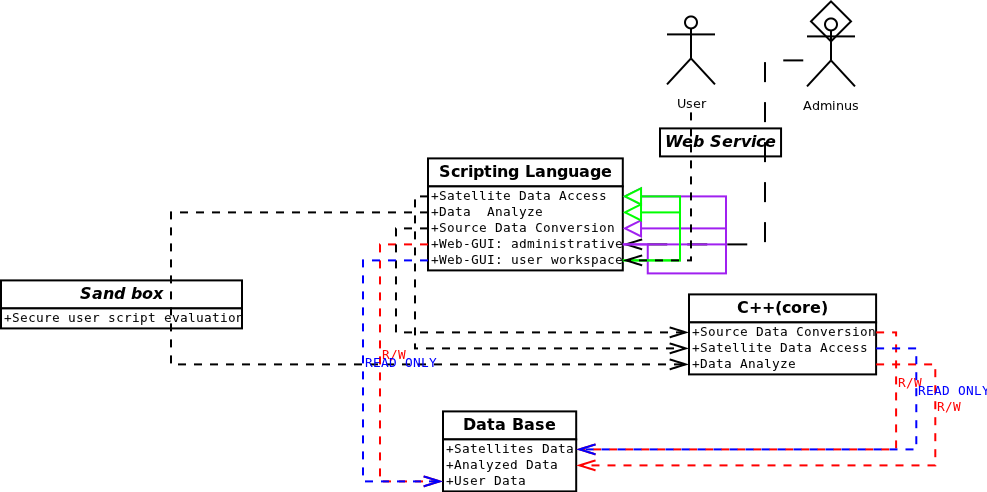
\includegraphics[height=0.50\textwidth]{presentation_1_scheme_1.png}
\end{frame}

% --------------------------------------------------- Slide -------------------
\subsection{C++ (core)}
\subsubsection{Source Data Conversion}
\begin{frame}
    \frametitle{Source Data Conversion}
    \begin{itemize}
        \item \colorbox{light-blue}{\underline{Опис}:} Перетворення сировинних данних супутника та надає можливість їх збереження.
        \item \colorbox{light-blue}{\underline{Мета}:} Забезпечення інструментарію написання парсерів та конверторів данних для нових космічних проектів.
    \end{itemize}
\end{frame}

% --------------------------------------------------- Slide -------------------
\subsubsection{Satellite Data Access}
\begin{frame}
    \frametitle{Satellite Data Access} 
    \begin{itemize}
        \item \colorbox{light-blue}{\underline{Опис}:} Отримання та фільтрування данних з супутникових проектів.
        \item \colorbox{light-blue}{\underline{Мета}:} Забезпечення простого інтерфейсу доступу до данних супутникових проектів.
    \end{itemize}
\end{frame}

% --------------------------------------------------- Slide -------------------
\subsubsection{Data Analyze}
\begin{frame}
    \frametitle{Data Analyze}
    \begin{itemize}
        \item \colorbox{light-blue}{\underline{Опис}:} Пакет математичних функцій та перетворень над масивами супутникових вимірів.
        \item \colorbox{light-blue}{\underline{Мета}:} Забезпечення аналізу, відображення та візуалізації данних.
    \end{itemize}
\end{frame}

% --------------------------------------------------- Slide -------------------
\subsection{Scripting Language}
\subsubsection{Source Data Conversion}
\begin{frame}
    \frametitle{Source Data Conversion}
    \begin{itemize}
        \item \colorbox{light-blue}{\underline{Опис}:} Перетворення та збереження сирцевих данних супутникових проектів.
        \item \colorbox{light-blue}{\underline{Мета}:} Забезпечення перетворення та збереження данних супутникових проектів. Обмеження конкретного парсеру збереженням данних саме цього супутникового проекту.
    \end{itemize}
\end{frame}

% --------------------------------------------------- Slide -------------------
\subsubsection{Satellite Data Access}
\begin{frame}
    \frametitle{Satellite Data Access}
    \begin{itemize}
        \item \colorbox{light-blue}{\underline{Опис}:} Доступ до данних супутникових проектів з обмеженням лише на читання.
        \item \colorbox{light-blue}{\underline{Мета}:} Надання зручного доступу та фільтрації данних без можливості зміни їх джерела.
    \end{itemize}
\end{frame}

% --------------------------------------------------- Slide -------------------
\subsubsection{Data  Analyze}
\begin{frame}
    \frametitle{Data  Analyze}
    \begin{itemize}
        \item \colorbox{light-blue}{\underline{Опис}:} Обгортка С++ модулю аналізу данних, що забезпечує гручний і зрозумілий потік данних крізь аналізатори.
        \item \colorbox{light-blue}{\underline{Мета}:} Побудова зручного API для аналізу данних та генерації простих скриптів у графічному режимі.
        \item \colorbox{light-blue}{\underline{Нагальні задачі}:} 
        \begin{itemize}
            \item Зручна модель представлення данних.
            \item Застосування Method Chaining або Fluent Interface, як моделі оперування данними.
        \end{itemize}
    \end{itemize}
\end{frame}

% --------------------------------------------------- Slide -------------------
\subsubsection{Web-GUI (administrative)}
\begin{frame}
    \frametitle{Web-GUI (administrative)}
    \begin{itemize}
        \item \colorbox{light-blue}{\underline{Опис}:} Частина користувацького інтерфейсу, що забезпечує керування користувацькими данними, супутниковими проектами, процесом постачання та аналізу данних.
        \item \colorbox{light-blue}{\underline{Мета}:} Сворення керівного модулю.
        \item \colorbox{light-blue}{\underline{Функції керування}:} 
        \begin{itemize}
            \item Користувацькими данними/запитами.
            \item Супутниковими проектами.
            \item Процесом обробки супутникових проектів.
        \end{itemize}
    \end{itemize}
\end{frame}

% --------------------------------------------------- Slide -------------------
\subsubsection{Web-GUI (user workspace)}
\begin{frame}
    \frametitle{Web-GUI (administrative)}
    \begin{itemize}
        \item \colorbox{light-blue}{\underline{Опис}:} Частина користувацького інтерфейсу, що представляє доступ до статичної інформації про проект та до робочого(дослідницького) простору.
        \item \colorbox{light-blue}{\underline{Мета}:} Забезпечення доступу до матеріалів проекту.
    \end{itemize}
\end{frame}

% --------------------------------------------------- Slide -------------------
\section{Software}
\begin{frame}
    \begin{center}
        \huge \ttfamily Засоби реалізації поставлених задач
    \end{center}
\end{frame}

% --------------------------------------------------- Slide -------------------
\subsection{Languages \& Frameworks}
\begin{frame}
    \begin{itemize}
        \item \colorbox{light-blue}{C++: STL/Boost/GSL} Написання наукомісткої частини, що включатиме фільтри, функції та методи аналізу, стандартні алгоритми.
        \item \colorbox{light-blue}{PostgreSQL} База данних, центральне сховище супутникових данних, тимчасових та користувацьких данних.
        \item \colorbox{light-blue}{Gearman} Контроль та розподіл виконання завдань між кількома потоками/серверами.
        \item \colorbox{light-blue}{JS: JQuery} Інтерактивна взаємодія з користувачем на клієнтській стороні.
    \end{itemize}
\end{frame}

% --------------------------------------------------- Slide -------------------
\subsection{Script Language}
\begin{frame}
    \frametitle{Скриптова мова}
    Основна проблема, що виникає при виборі - безпечне виконання на стороні серверу. Варіанти.
    \begin{itemize}
        \item \colorbox{light-blue}{Python / Virtualization} Можливість безпечного запуску сторонніх скриптів є небажанною з версії 2.6 і вимкнена в 3.0 через проблеми безпеки.
        \item \colorbox{light-blue}{JavaScript / Node.js} Можливе виконання на серверній стороні за допомогою Node.js, що працює на базі v8(Google). Безпечне виконання на базы налаштувань та обмежень Node.js.
    \end{itemize}
\end{frame}

\begin{frame}
    \frametitle{Наслідки використання}
    \begin{itemize}
        \item \colorbox{light-blue}{Python / Virtualization} Використання Django та супунього серверу для побудови веб-інтерфейсу. Підняття віртуальнох машини для виконання скриптів.
        \item \colorbox{light-blue}{JavaScript / Node.js} Використання PHP / Yii для написання веб-інтерфейсу. Підняття Apache / nginx серверів для виконання PHP.
    \end{itemize}
\end{frame}

% --------------------------------------------------- Slide -------------------
\section{Documentation}
\begin{frame}
    \begin{center}
        \huge \ttfamily Документування
    \end{center}
\end{frame}

% --------------------------------------------------- Slide -------------------
\subsection{Developer to developer}
\begin{frame}
    \frametitle{Розробник-розробнику}
    Має вигляд:
    \begin{itemize}
        \item Набір UML схем, що спростять розуміння архітектури проекту, та певних складних або вузьких елементів програмної реалізації чи алгоритмів.
        \item Вікі-сторінки з описом та обговоренням ідей алгоритмів, реалізації.
        \item Система документації та обговорення багів.
        \item Система опису життя та розвитку проекту: мінорні та мажорні версії, milestones і т.п.
    \end{itemize}
\end{frame}

% --------------------------------------------------- Slide -------------------
\subsection{Developer to user}
\begin{frame}
    \frametitle{Розробник-користувачу: API классів({\it Class Reference})}
    \begin{itemize}
        \item Генерується з програмного коду за допомогою Doxygen.
        \item Містить опис усіх функцій та їх вхідни та вихідних параметрів.
        \item Містить важливі приклади використання.
        \item Коротко та просто.
    \end{itemize}
\end{frame}

% --------------------------------------------------- Slide -------------------
\begin{frame}
    \frametitle{Розробник-користувачу: Ознайомлюючий ввід({\it Definitive guide})}
    \begin{itemize}
        \item Докладний огляд усіх базових принципів та ідей за прикладами та ліричними відступами.
        \item Огляд ідей та ідіом, що варто використовувати при роботі з інструментарем проекту.
        \item Приклади розв’язку задач, що часто виникають в практиці.
    \end{itemize}
\end{frame}

% --------------------------------------------------- Slide -------------------
\subsection{User to user}
\begin{frame}
    \frametitle{Користувач-користувачу: Користувацькі статті({\it Wiki pages})}
    \begin{itemize}
        \item Опис розв’язку складних, нестандартних проблем.
    \end{itemize}
\end{frame}

% --------------------------------------------------- Slide -------------------
\section{Conclusions}
\subsection{Questions}
\begin{frame}
    \frametitle{Нагальні питання}
    \begin{itemize}
        \item Вибір скриптовох мови та супутнього пакету проблем до кожної з них
        \item Створення списку математичних функцій, фільтрів що будуть реалізовуватись
        \item Створення типу данних для передачі та зручного трансферу та їх перетворення
    \end{itemize}
\end{frame}

\end{document}

